\documentclass{article}

\usepackage{graphicx}
\usepackage{tikz}
\usepackage{tikzsymbols}
\usetikzlibrary{calc,patterns,shapes.geometric}
\pagestyle{empty}
\usepackage[margin=0pt]{geometry}
\geometry{papersize={14in,12in}}

\def\centerarc[#1](#2)(#3:#4:#5){\draw[#1] ($(#2)+({#5*cos(#3)},{#5*sin(#3)})$) arc (#3:#4:#5);}

\begin{document}
	\begin{figure}
		\centering
		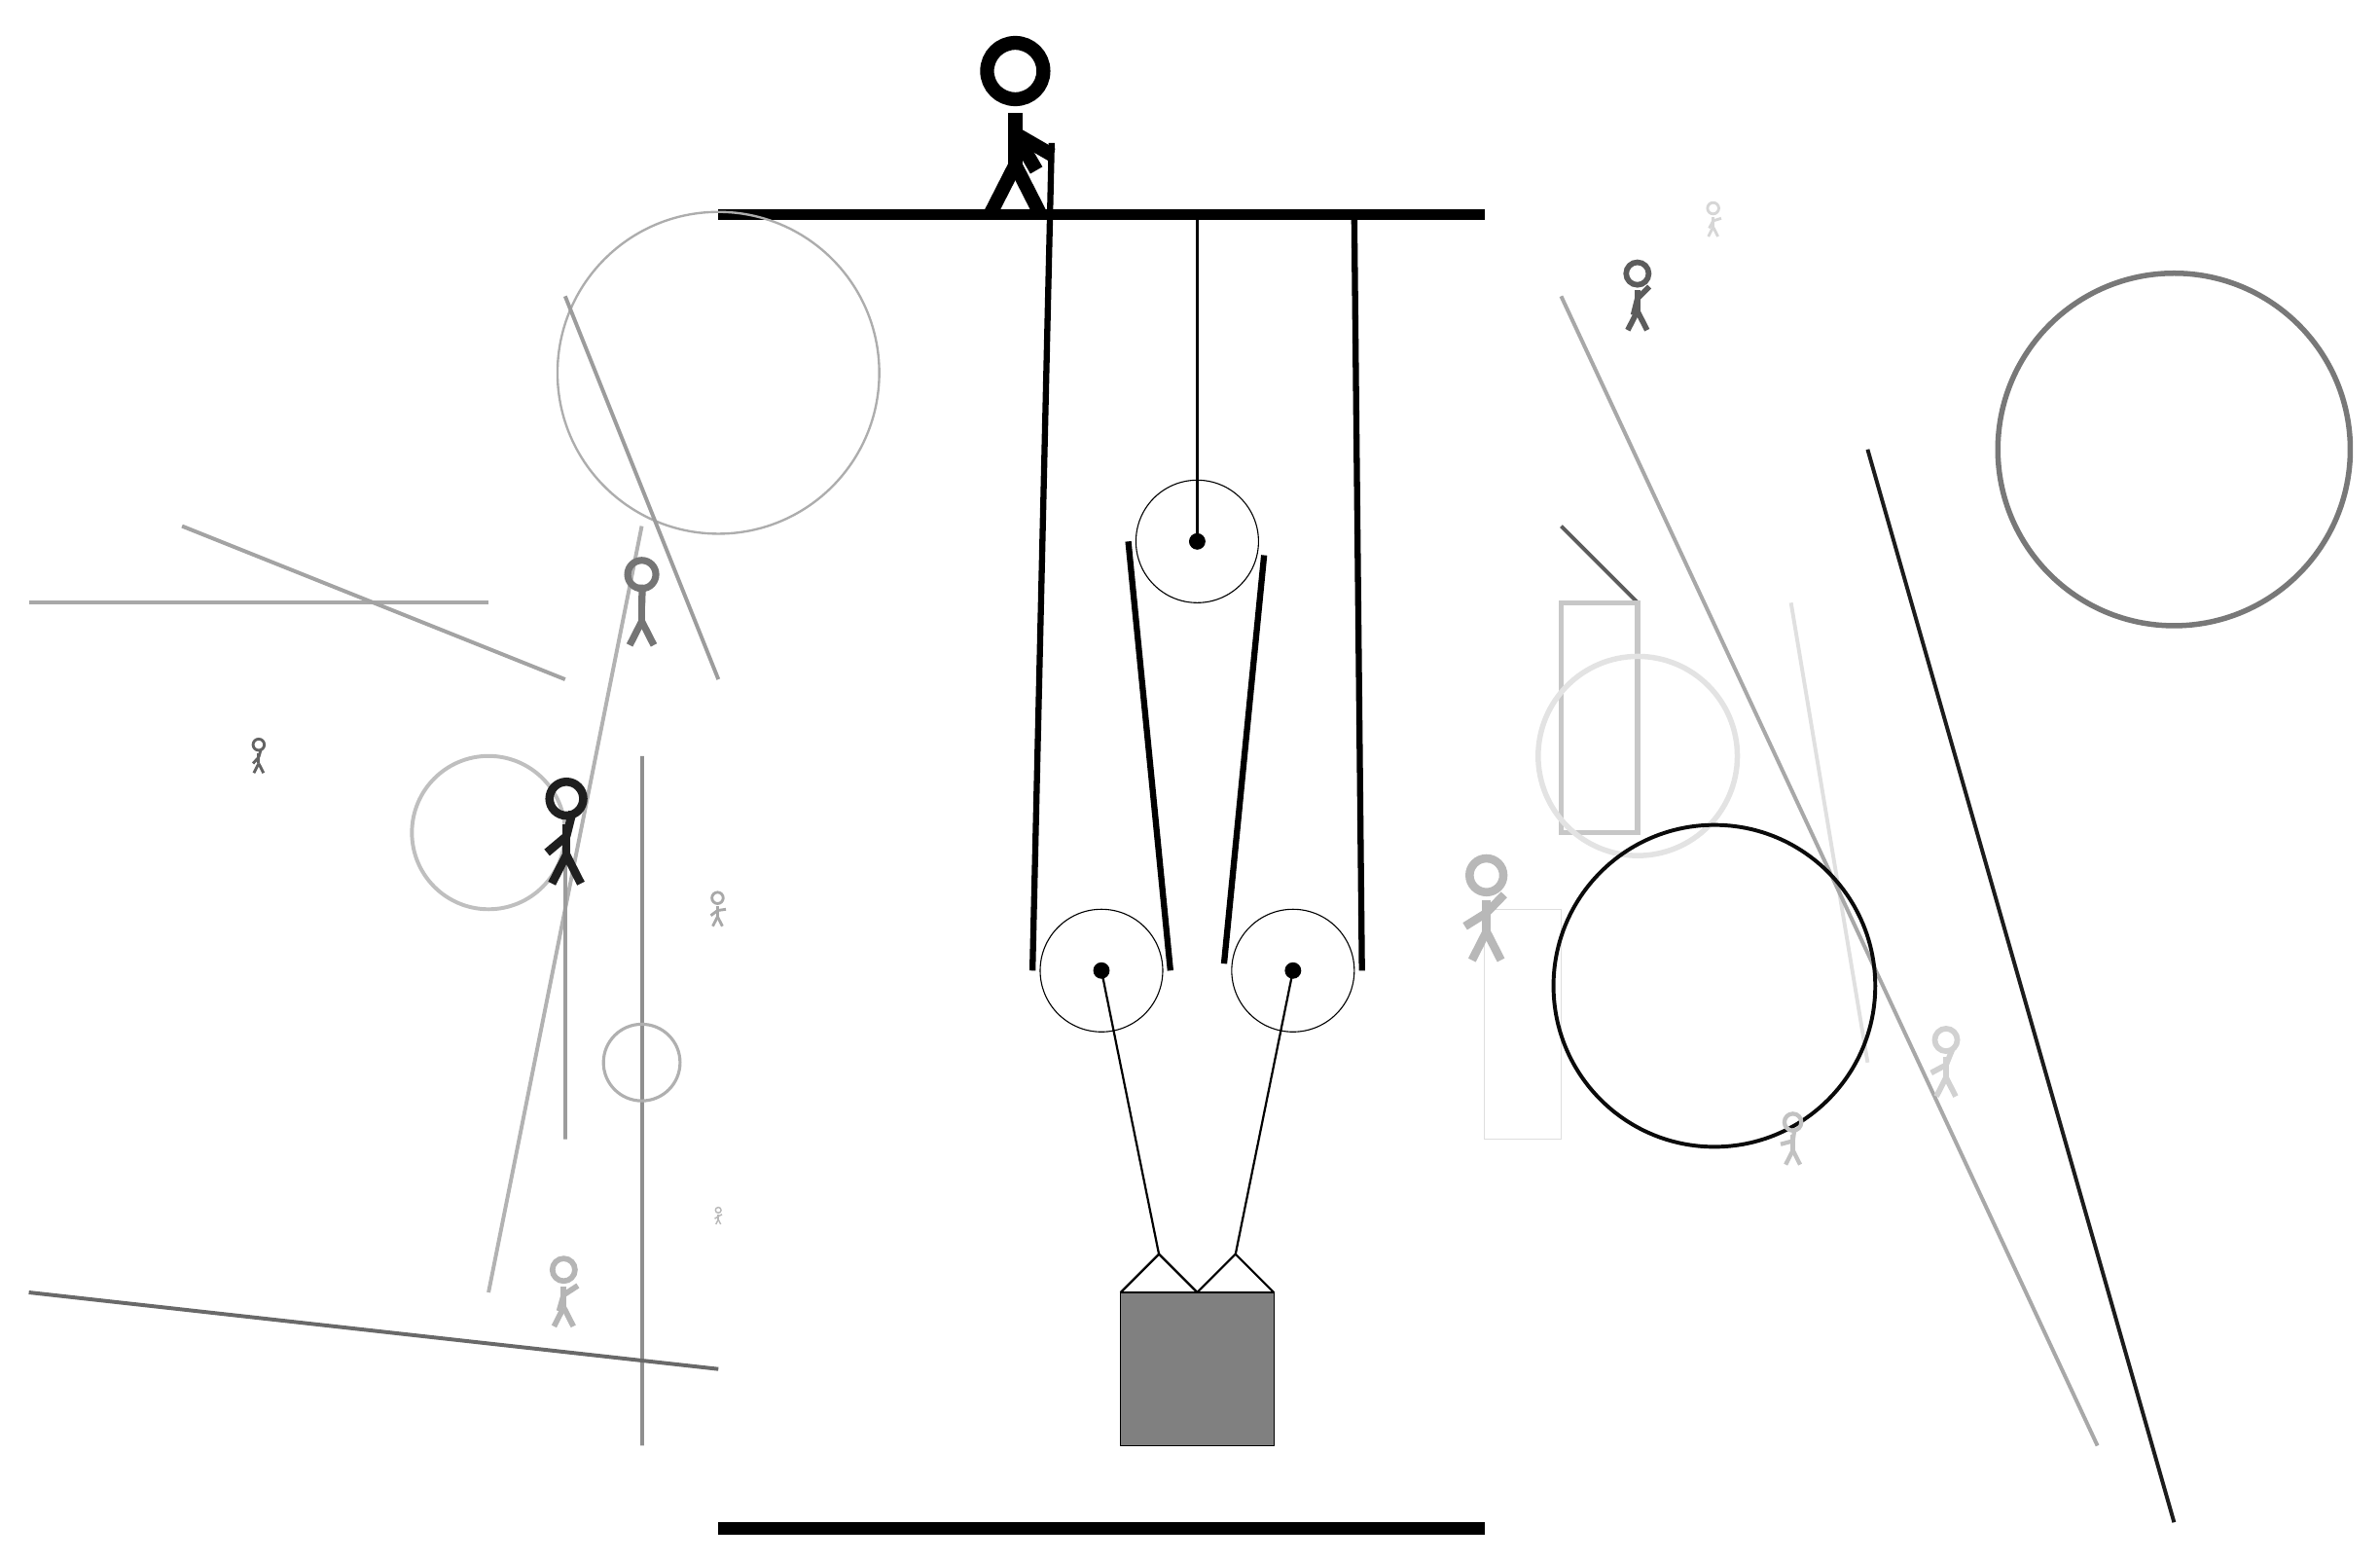
\begin{tikzpicture}
			%%%%% START %%%%%
			
			\draw[fill=black] (-4, 14) rectangle (6, 14.125);
			
			\draw (1, 4.2) circle (0.8);
			\draw[fill=black] (1, 4.2) circle (0.1);
			
			\draw (2.25, 9.8) circle (0.8);
			\draw[fill=black] (2.25, 9.8) circle (0.1);
			\draw[thick] (2.25, 9.8) -- (2.25, 14);
			
			\draw (3.5, 4.2) circle (0.8);
			\draw[fill=black] (3.5, 4.2) circle (0.1);
			
			\draw[thick] (3.5, 4.2) -- (2.75, 0.5);
			\draw[thick] (1, 4.2) -- (1.75, 0.5);
			\draw[thick]  (1.25, 0) -- (1.75, 0.5) -- (2.25, 0);
			\draw[thick]  (2.25, 0) -- (2.75, 0.5) -- (3.25, 0);
			\draw[fill=black!50] (1.25, 0) rectangle (3.25, -2);
			
			\draw[line width=0.8mm] (0.35, 15) --  (0.1, 4.2);
			\centerarc[line width=0.8mm](1, 4.2)(180:360:0.9);
			\draw[line width=0.8mm] (1.9, 4.2) -- (1.35, 9.8);
			\centerarc[line width=0.8mm](2.25, 9.8)(-20:180:0.9);
			\draw[line width=0.8mm](3.123, 9.62) -- (2.6, 4.29);
			\centerarc[line width=0.8mm](3.5, 4.2)(160:360:0.9);
			\draw[line width=0.8mm](4.4, 4.2) -- (4.3, 14);
			
			\draw[line width=0.5mm, color=black!44] (-5, 7) rectangle (-5, -2);
			
			\draw[line width=0.5mm, color=black!59](-4, -1) -- (-13, 0);
			\draw [line width=0.4mm, color=black!31](-5, 3) circle (0.5);
			\node[line width=0.4mm, color=black!28] at (-4, 1) {\Strichmaxerl[1][33][28]};
			
			\draw [line width=0.3mm, color=black!32](-4, 12) circle (2.1);
			
			\node[line width=0.7mm, color=black!61] at (-10, 7) {\Strichmaxerl[2][48][74]};
			\draw[line width=0.5mm, color=black!34](-7, 9) -- (-13, 9);
			
			\draw[line width=0.5mm, color=black!64](7, 10) -- (8, 9);
			\draw[line width=0.2mm, color=black!13] (7, 2) rectangle (6, 5);
			
			\draw[line width=0.5mm, color=black!30](-7, 0) -- (-5, 10);
			\node[line width=0.6mm, color=black!54] at (-5, 9) {\Strichmaxerl[5][90][88]};
			\node[line width=0.5mm, color=black!29] at (-6, 0) {\Strichmaxerl[4][74][33]};
			\draw[line width=0.5mm, color=black!89](11, 11) -- (15, -3);
			
			\node[line width=0.2mm, color=black!34] at (-4, 5) {\Strichmaxerl[2][37][8]};
			\node[line width=0.5mm, color=black!28] at (6, 5) {\Strichmaxerl[6][32][46]};
			\draw[line width=0.7mm, color=black!22] (8, 9) rectangle (7, 6);
			
			\draw[line width=0.5mm, color=black!12](10, 9) -- (11, 3);
			\draw[line width=0.5mm, color=black!34](7, 13) -- (14, -2);
			\draw [line width=0.7mm, color=black!11](8, 7) circle (1.3);
			\draw[line width=0.5mm, color=black!36](-6, 8) -- (-11, 10);
			\draw [line width=0.5mm, color=black!25](-7, 6) circle (1.0);
			
			\node[line width=0.4mm, color=black!18] at (12, 3) {\Strichmaxerl[4][28][68]};
			\draw[line width=0.5mm, color=black!39](-6, 13) -- (-4, 8);
			\node[line width=0.7mm, color=black!16] at (9, 14) {\Strichmaxerl[2][62][17]};
			\node[line width=0.4mm, color=black!64] at (8, 13) {\Strichmaxerl[4][76][45]};
			
			\draw[line width=0.5mm, color=black!39] (-6, 6) rectangle (-6, 2);
			\draw [line width=0.5mm, color=black!96](9, 4) circle (2.1);
			\draw [line width=0.7mm, color=black!53](15, 11) circle (2.3);
			\node[line width=0.5mm, color=black!88] at (-6, 6) {\Strichmaxerl[6][40][76]};
			\node[line width=0.4mm, color=black!24] at (10, 2) {\Strichmaxerl[3][15][82]};
			
			\node at (-0.07, 15.2) {\Strichmaxerl[10][120][-30]};
			
			\draw[fill=black] (-4, -3) rectangle (6, -3.15);
			
			%%%%% END %%%%%
		\end{tikzpicture}
	\end{figure}	
\end{document}